% Separate condensed review candidate; the original main.tex and PDF are unchanged.
% Compile with: pdflatex -jobname=DT081A_Lab3_Report_SHORT_REVIEW main_short.tex
\documentclass[10pt,a4paper]{article}
\usepackage[T1]{fontenc}
\usepackage{lmodern}
\usepackage[margin=20mm]{geometry}
\usepackage{graphicx,amsmath,booktabs,caption,float,listings,titlesec,hyperref}
\hypersetup{hidelinks,pdftitle={DT081A Lab 3 - Condensed Review Candidate},
  pdfauthor={Yacoub Dawli and Obid Alrhman Aljabi}}
\graphicspath{{../figures/}}
\setlength{\parindent}{0pt}
\setlength{\parskip}{2pt}
\setlength{\intextsep}{5pt}
\setlength{\textfloatsep}{5pt}
\titleformat{\section}{\large\bfseries}{\thesection}{0.6em}{}
\titleformat{\subsection}{\normalsize\bfseries}{\thesubsection}{0.6em}{}
\titlespacing*{\section}{0pt}{6pt}{3pt}
\titlespacing*{\subsection}{0pt}{5pt}{2pt}
\captionsetup{font=small,labelfont=bf,skip=3pt}
\lstset{basicstyle=\ttfamily\fontsize{8.5}{10}\selectfont,
  columns=fullflexible,keepspaces=true,showstringspaces=false,
  aboveskip=1pt,belowskip=2pt}
\setlength{\emergencystretch}{1em}
\clubpenalty=10000
\widowpenalty=10000
\raggedbottom
\pagestyle{plain}

\begin{document}
\begin{center}
{\large DT081A - Signal and Image Processing}\\[2pt]
{\large\bfseries Lab 3 Report - Condensed Review Candidate}\\[3pt]
Yacoub Dawli (Jakob) --- \texttt{yada2100@student.miun.se}\\
Obid Alrhman Aljabi --- \texttt{obal2302@student.miun.se}\\[2pt]
{\small Original report: 24 October 2026. Condensed candidate: 29 October 2026.}
\end{center}
\vspace{-5pt}

\section{Introduction}
We studied pixel transforms, colour reduction, filtering, Fourier analysis,
histograms and morphology. Numerical results helped compare brightness,
detail, noise, execution time and memory use.

\section{Experimental Setup}
The verified experiments used Python, NumPy, OpenCV 5.0.0 and Matplotlib.
We used the course \(512\times512\) peppers TIFF because \texttt{ManWoman.png}
was unavailable; the lab permits other images. BGR was converted to RGB for
display, with grayscale and synthetic images where needed. Experiments were
not rerun for this candidate.

\section{Results and Analysis}
\subsection{Gamma Correction}
\textbf{Q1.1.} We used \(255(I/255)^\gamma\). At \(\gamma=2.0\),
Table~\ref{tab:gamma} shows darker outputs; \texttt{uint8} conversion drops
fractional parts.

\begin{table}[H]
\centering\small
\caption{Gamma calculation, \(\gamma=2.0\).}\label{tab:gamma}
\begin{tabular}{rrr}\toprule
Input & Before integer conversion & \texttt{uint8} output\\\midrule
64 & 16.063 & 16\\
128 & 64.251 & 64\\
192 & 144.565 & 144\\\bottomrule
\end{tabular}
\end{table}

\textbf{Q1.2.} With \(\gamma=2.2\), mean intensity fell from 120.22 to 61.00.
The image darkened and its histogram moved lower, with gaps from integer
conversion (Figure~\ref{fig:gamma}). This nonlinear change relates to unequal
visual sensitivity, but is not an exact logarithmic eye model. We used the
lab's \(\gamma\), not camera pre-correction's \(1/\gamma\).

\begin{figure}[H]
\centering
% Preserve both histogram axes and their original shared scales.
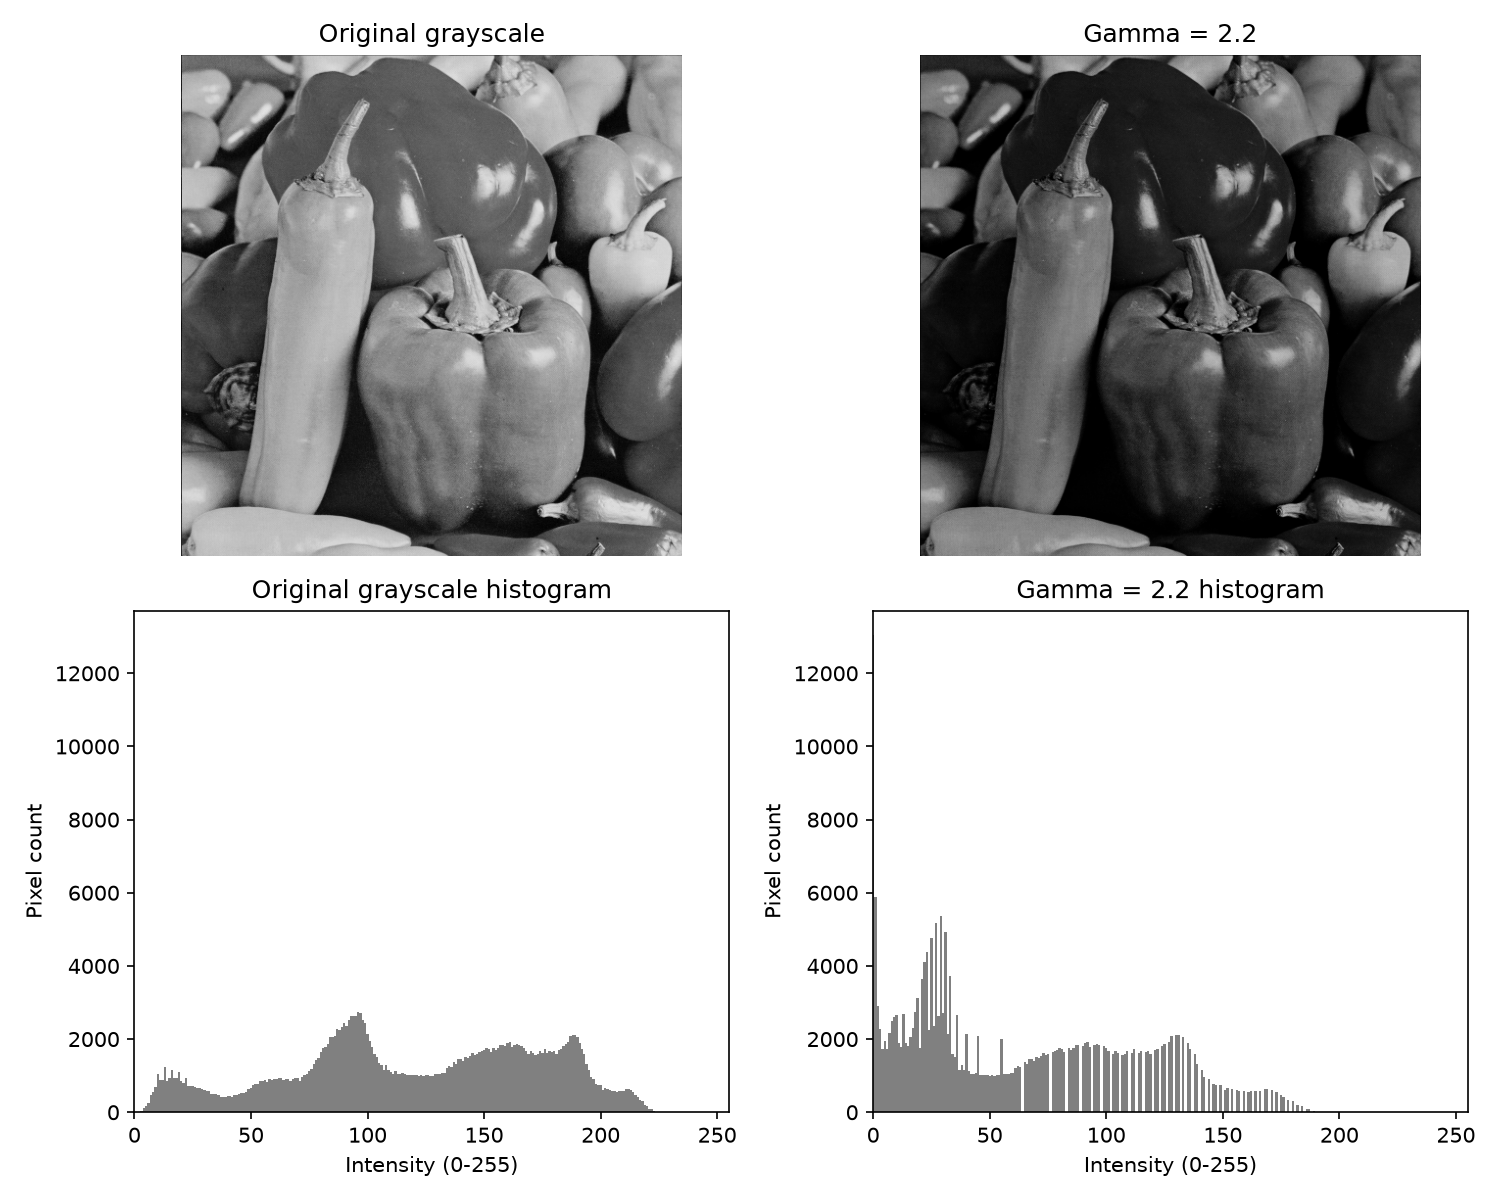
\includegraphics[trim=0 0 0 273.6bp,clip,width=\linewidth]{section1_gamma_histograms.png}
\caption{Original and gamma-2.2 histograms. Axes and count scales are unchanged.}
\label{fig:gamma}
\end{figure}

\subsection{Colorspaces}
\textbf{Q2.1.} OpenCV's order is Y, Cr, Cb, with
\(Y\approx0.299R+0.587G+0.114B\). All channels started at 0; Y/R/G/B maxima
were 228/231/237/229, and standard deviations 53.88/45.17/75.05/44.29.
G was widest; Y lay between G and R/B. R had many high values and B mostly low
ones. Y simplifies brightness-edge detection to one channel, but can miss
equal-brightness colour boundaries.

\textbf{Q2.2.} We kept Y and reduced both chroma dimensions by factors 2, 4 and
8, using area reduction and linear reconstruction. Factor 2 changes \(3N\)
samples to \(N+N/4+N/4=1.5N\): 786,432 to 393,216 bytes, saving 50\%.
Factors 4/8 need 294,912/270,336 bytes, saving 62.5/65.625\%.
These are stored channel samples before display reconstruction, not compressed
files. Factor 2 looked close; factor 4 softened colour boundaries and factor 8
showed clearer blending, while Y detail remained.

\subsection{Quantization and Sampling}
\textbf{Q3.1.} RGB integer division by 16 gave 16 possible levels per channel,
displayed as \(0,16,\ldots,240\). Only 15 were occupied because no input reached
240; smooth colours became slightly stepped and darker. Packed 4-bit storage
would give \(2{:}1\) reduction, or 50\% saving: 393,216 versus 786,432 bytes.
The actual \texttt{uint8} array still occupied 786,432 bytes.

\textbf{Q3.2.} Grayscale division by 32 grouped 32 input intensities into each
of eight levels, displayed as \(0,32,\ldots,224\). All eight were occupied;
the last held only 29 pixels. Both histograms counted 262,144 pixels.
Combining nearby intensities caused banding and lost shading and texture,
although outlines remained clear.

\subsection{Convolution and Edge Detection}
\textbf{Q4.1.} We compared matching Gaussian kernels at \(\sigma=1\), using
float64 output and \texttt{BORDER\_REFLECT\_101}, after warm-up
(Table~\ref{tab:times}). Separable filtering was faster only at \(5\times5\);
ordinary 2D was slightly faster at 11 and 21. Costs fall from \(k^2\) to about
\(2k\) weights per pixel, potentially helping large kernels, but library
implementation affects real speed. Both outputs looked alike, differing by
at most about 0.000002 intensity units.

\begin{table}[H]
\centering\small
\caption{Recorded average times; loading and plotting excluded.}\label{tab:times}
\begin{tabular}{lrrr}\toprule
Task (first / second method) & Runs & First (ms) & Second (ms)\\\midrule
Gaussian \(5\times5\) (2D / separable) & 30 & 5.420 & 1.429\\
Gaussian \(11\times11\) (2D / separable) & 30 & 9.880 & 10.455\\
Gaussian \(21\times21\) (2D / separable) & 30 & 23.481 & 24.022\\
Brightness (NumPy / loops) & 5 & 2.040 & 468.915\\
Log transform (direct / lookup) & 30 & 9.469 & 2.468\\\bottomrule
\end{tabular}
\end{table}

\textbf{Q4.2.} Our \(3\times3\) Sobel function used \texttt{dx=0, dy=1}.
Absolute top-to-bottom brightness changes highlighted horizontal boundaries,
while long vertical sides were weaker. The \texttt{dx=1, dy=0} comparison
favoured vertical edges; curved edges appeared in both.

\textbf{Q4.3.} We combined signed derivatives as
\(G=\sqrt{G_x^2+G_y^2}\), normalizing a separate display copy to 0--255.
It showed more complete outlines and stems because it included both
directions; brighter pixels marked stronger edges (Figure~\ref{fig:frequency}, far right).

\subsection{Matrix Operations}
\textbf{Q5.1.} We stacked pixels, applied \(1.2(I-128)+128+20\), clipped to
0--255 and reshaped. NumPy and nested loops gave identical brighter images,
with some clipped highlights. NumPy was 229.82 times faster using unrounded
times (Table~\ref{tab:times}), avoiding a Python operation for every pixel.
Calculation, output creation and conversion were timed.

\textbf{Q5.2.} The stacked image has 262,144 values, so H has
\(262{,}144^2=68{,}719{,}476{,}736\) elements. Float32 needs
274,877,906,944 bytes (256 GiB); float64 needs 549,755,813,888 bytes (512 GiB),
where GiB is \(1024^3\) bytes. H was not allocated. Most entries would be zero;
keeping nine kernel weights and processing local neighbourhoods is more practical.

\subsection{Pixel-Based Processing}
\textbf{Q6.1.} Direct and 256-entry lookup versions gave identical
\texttt{uint8} images, range 0--240. Lookup was 3.84 times faster
(Table~\ref{tab:times}) because it reused results instead of recalculating
logarithms. Its separate 0.539 ms construction was excluded; applications
were warmed up and averaged over 30 calls.

\textbf{Q6.2.} Two logarithmic halves joined at 127.5, with strength 4.
The transfer curve was steeper centrally and flatter at both ends: input gaps
of 32 produced output gaps 17 (0--32), 64 (112--144), and 18 (223--255).
Thus middle shading separated more, while shadow/highlight differences
compressed. Dark gaps looked darker and light areas brighter. The full
mapping kept intensity order and mapped 0 to 0 and 255 to 255.

\subsection{Elementary Images}
\textbf{Q7.1.} Outer products of the teacher's vectors made \(16\times16\)
images: Ramp\(\times\)Ramp gave smooth two-direction changes;
Step\(\times\)Ramp a boundary plus a gradient; Step\(\times\)Step a sharp
lower-right block; Step\(\times\)Sine repeating columns in the lower half.
Their shared \(-1\) to 1 scale made zero middle gray.

\textbf{Q7.2.} Least squares fitted Step\(\times\)Ramp, Step\(\times\)Step and
Step\(\times\)Sine to an \(8\times8\) square at rows 8--15, columns 4--11
(zero-based). Weights were respectively 0.156058, 0.812731 and 0.688038;
MSE was 0.107400 on the 0--1 scale. The raw range was 0.000000--0.895961.
The horizontal boundary matched, but uneven interiors, wrong side edges and
outside bands remained: three patterns gave only a coarse fit (Figure~\ref{fig:shape}).

\begin{figure}[H]
\centering
\begin{minipage}[b]{45mm}\centering\small Target\\[2pt]
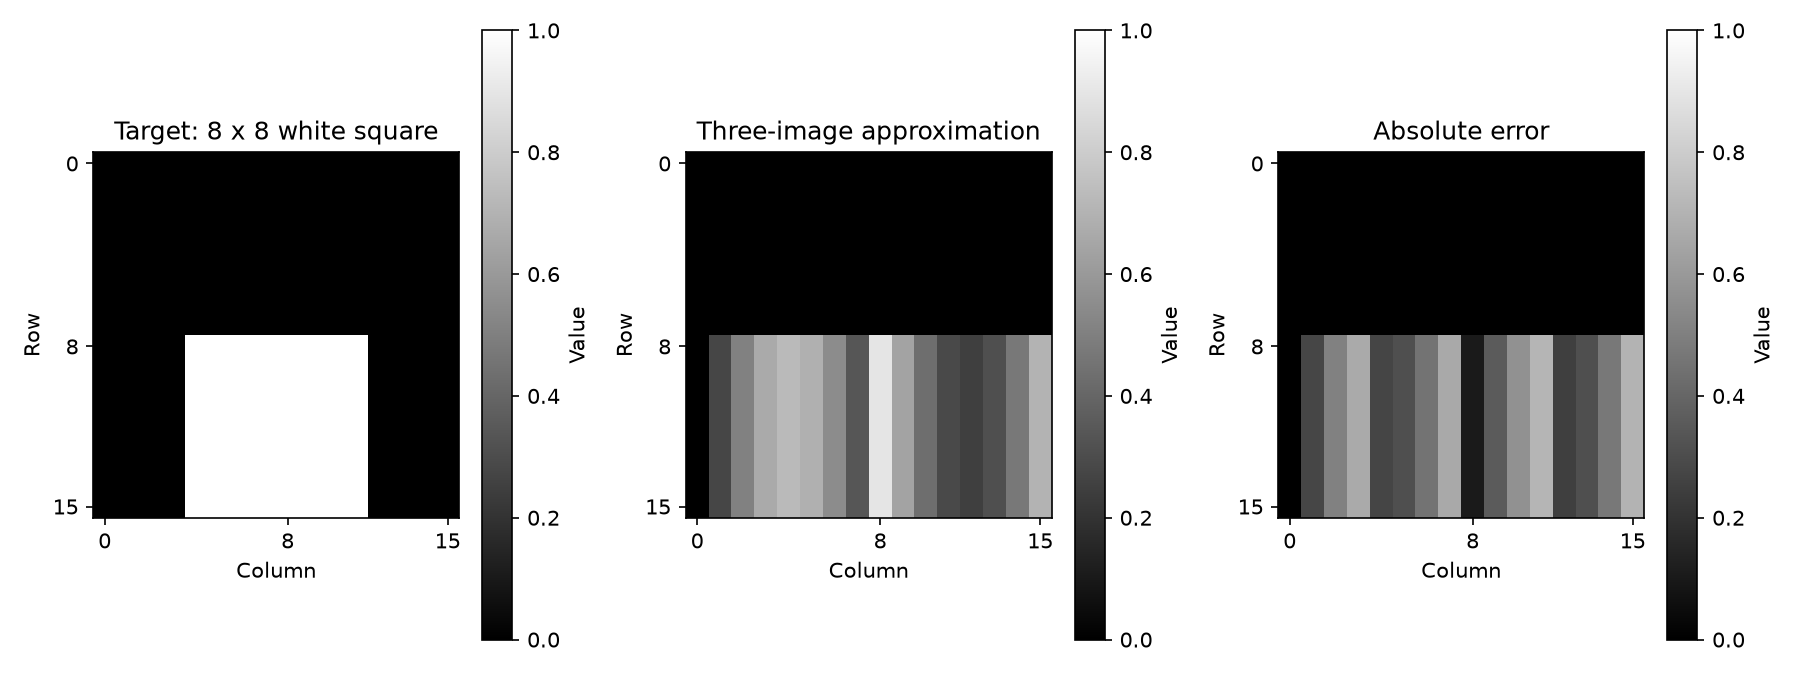
\includegraphics[trim=44.16bp 74.88bp 643.2bp 72.48bp,clip,width=\linewidth]{section7_shape_approximation.png}
\end{minipage}\hspace{8mm}
\begin{minipage}[b]{45mm}\centering\small Three-image fit\\[2pt]
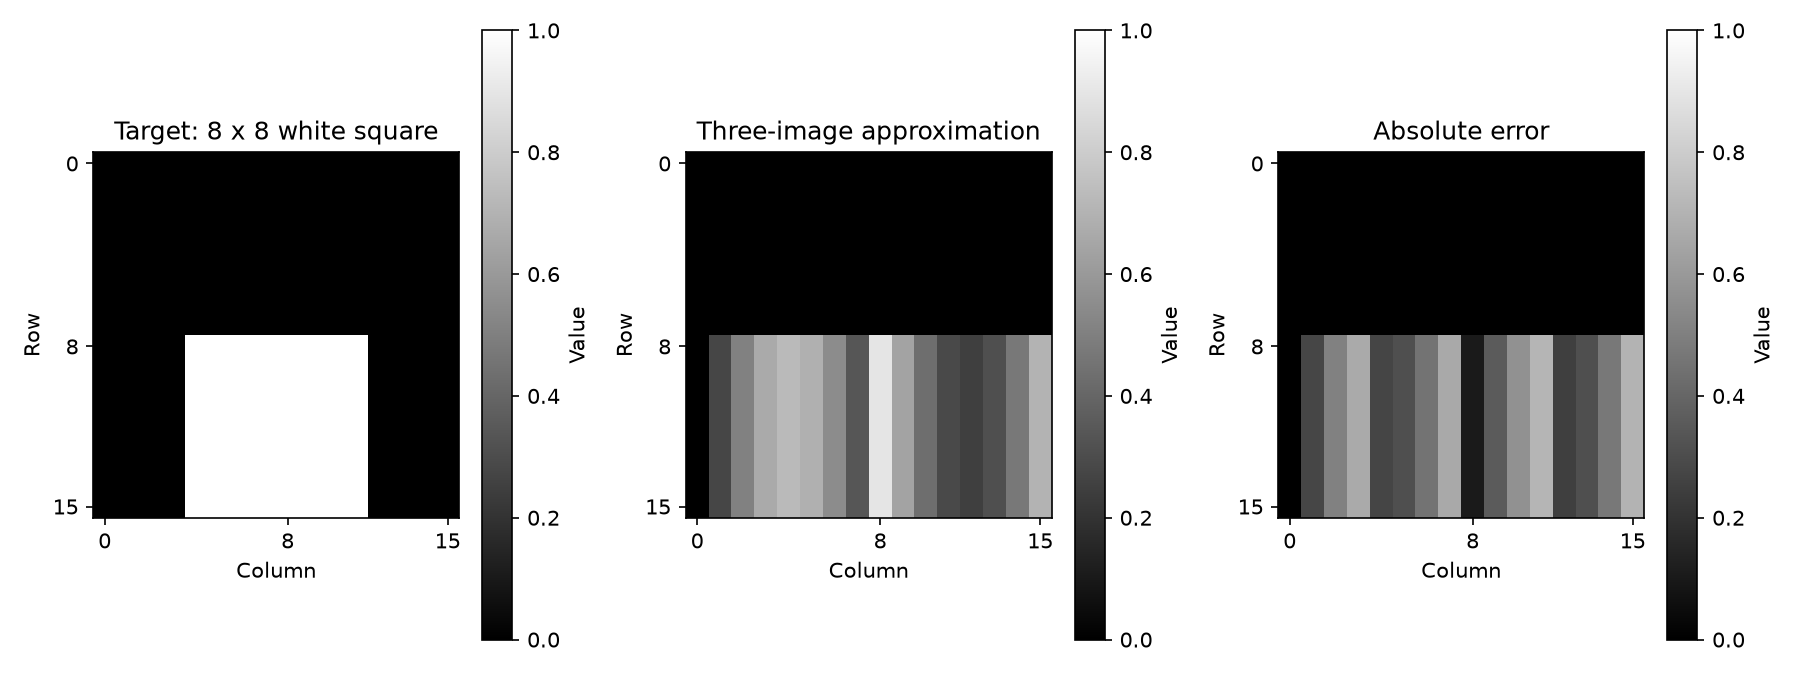
\includegraphics[trim=328.8bp 74.88bp 358.56bp 72.48bp,clip,width=\linewidth]{section7_shape_approximation.png}
\end{minipage}
\caption{Target and unchanged raw approximation. Both use black 0 to white 1.}
\label{fig:shape}
\end{figure}

\subsection{Transforms and Frequency Domain}
\textbf{Q8.1.} We displayed \texttt{log1p(abs(fftshift(fft2(gray))))}.
The bright centre held average brightness and slow changes; faster changes
lay farther out. Horizontal/vertical streaks included edges and border effects:
vertical edges contribute along horizontal frequency and vice versa.
Curves involve several directions. The FFT does not locate individual edges.

\textbf{Q8.2.} A circular low-pass mask kept radii below 40 bins in the
\(512\times512\) grid; inverse shifting and FFT returned its real part.
Main shapes remained, detail weakened and boundaries softened, with ringing
from the sharp cutoff (Figure~\ref{fig:frequency}). Raw values were
\(-17.078\) to 243.781; negatives displayed black without changing the data.

\textbf{Q8.3.} Floating-point original-minus-low-pass kept outlines, stems and
detail around near-zero smooth regions. The raw range was \(-155.400\) to
113.396; display limits were \(\pm155.400\), with zero middle gray.
Ringing remained. Low-pass plus high-pass recovered the original with maximum
error 0; the inverse FFT's largest imaginary part was \(6.172\times10^{-14}\).

\begin{figure}[H]
\centering
\begin{minipage}[b]{0.23\linewidth}\centering\small Low-pass\\0--255\\[2pt]
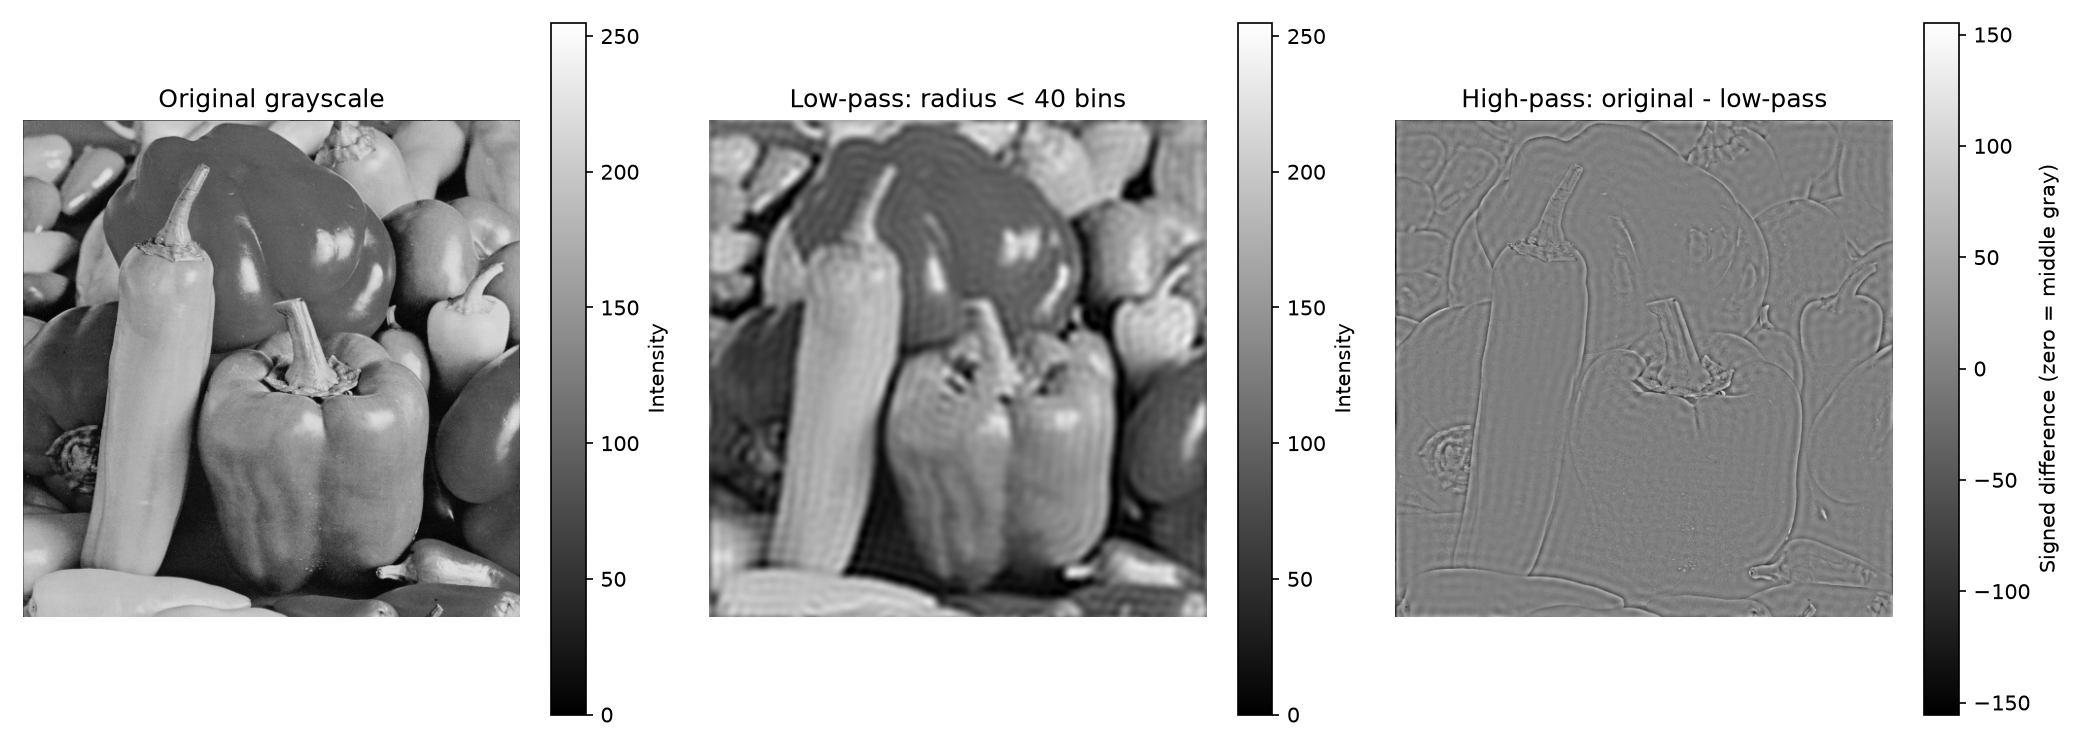
\includegraphics[trim=340.32bp 63.84bp 428.64bp 57.12bp,clip,width=\linewidth]{section8_frequency_filtering.png}
\end{minipage}\hfill
\begin{minipage}[b]{0.23\linewidth}\centering\small Signed high-pass\\zero middle gray\\[2pt]
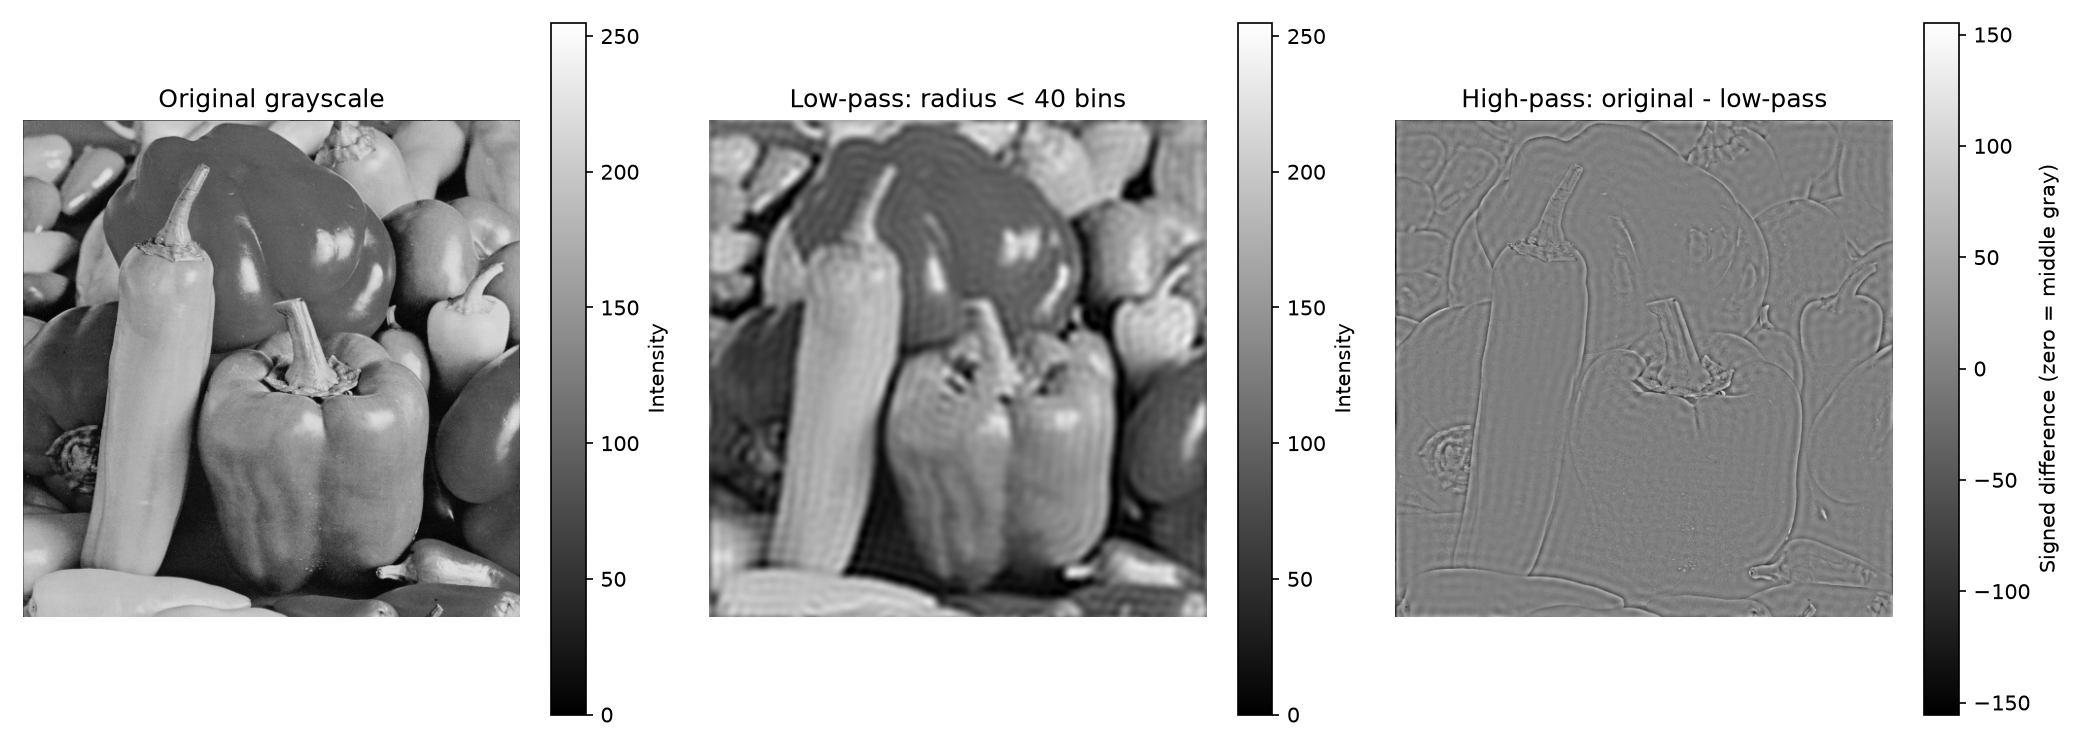
\includegraphics[trim=669.6bp 63.84bp 99.36bp 57.12bp,clip,width=\linewidth]{section8_frequency_filtering.png}
\end{minipage}\hfill
\begin{minipage}[b]{0.23\linewidth}\centering\small Morphological\\gradient\\[2pt]
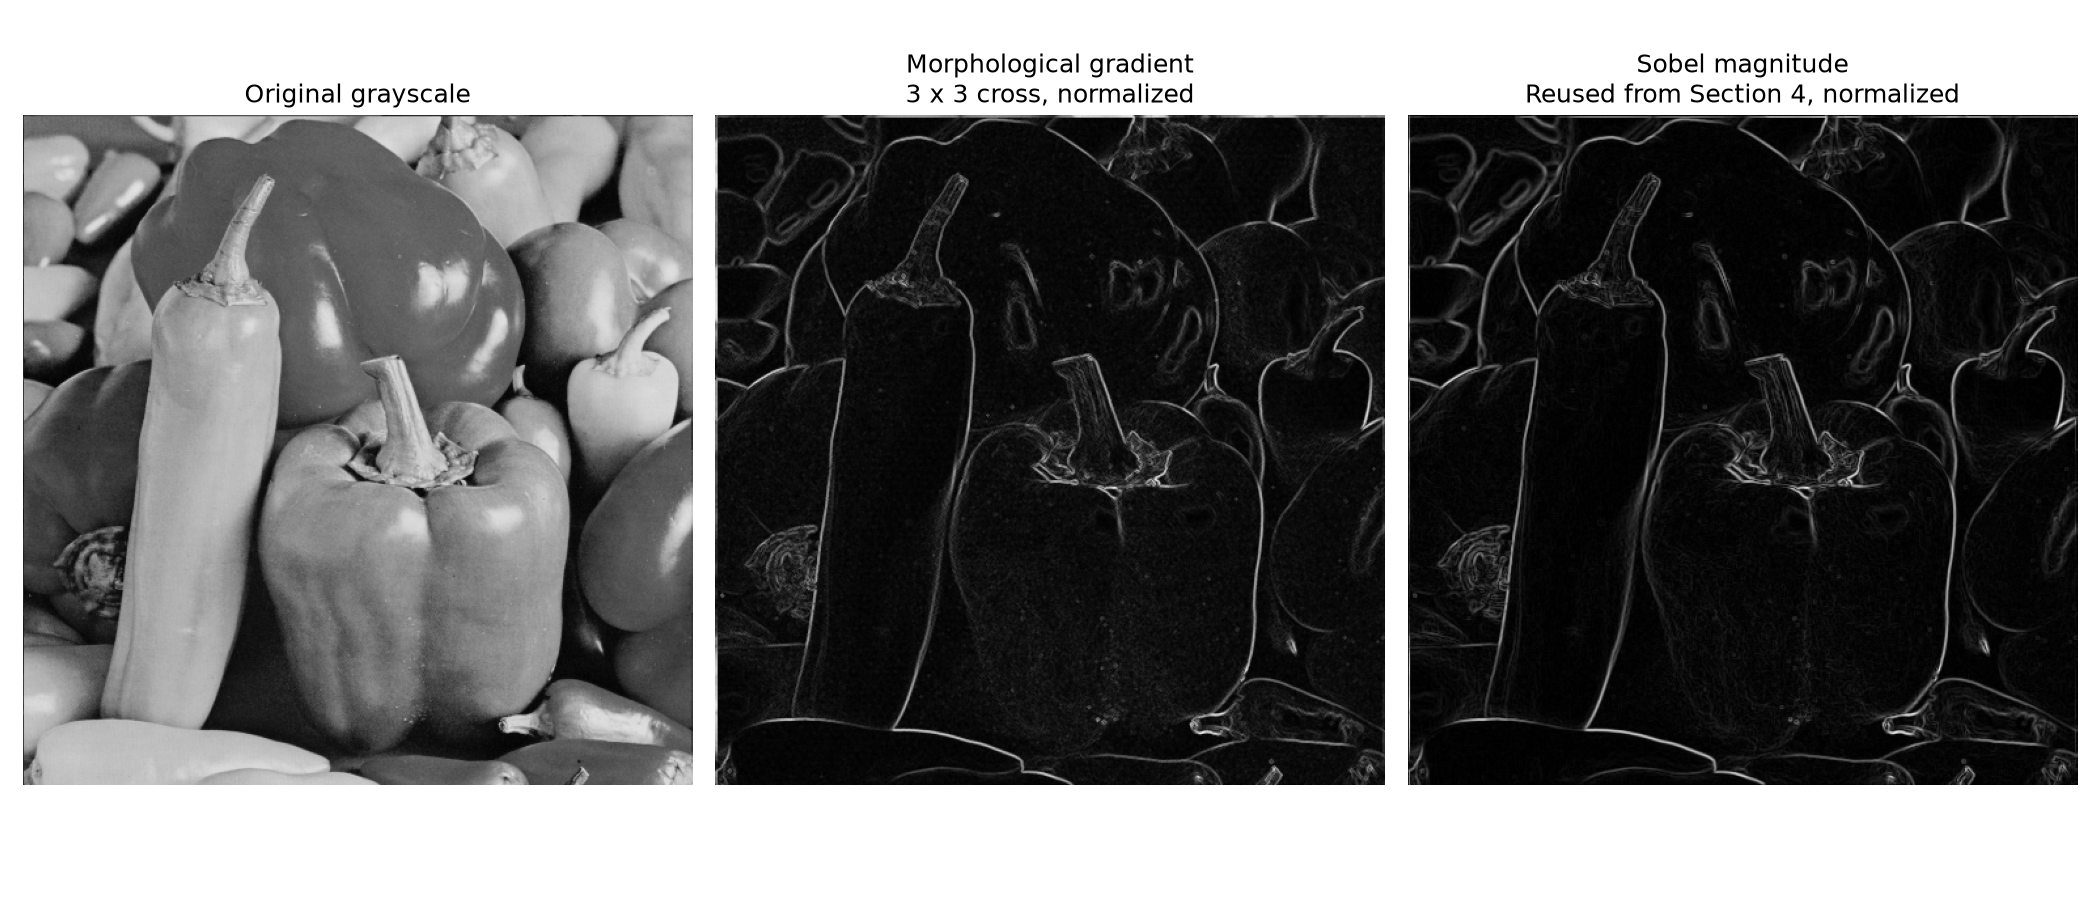
\includegraphics[trim=343.2bp 55.2bp 343.2bp 55.2bp,clip,width=\linewidth]{section11_gradient_comparison.png}
\end{minipage}\hfill
\begin{minipage}[b]{0.23\linewidth}\centering\small Sobel\\magnitude\\[2pt]
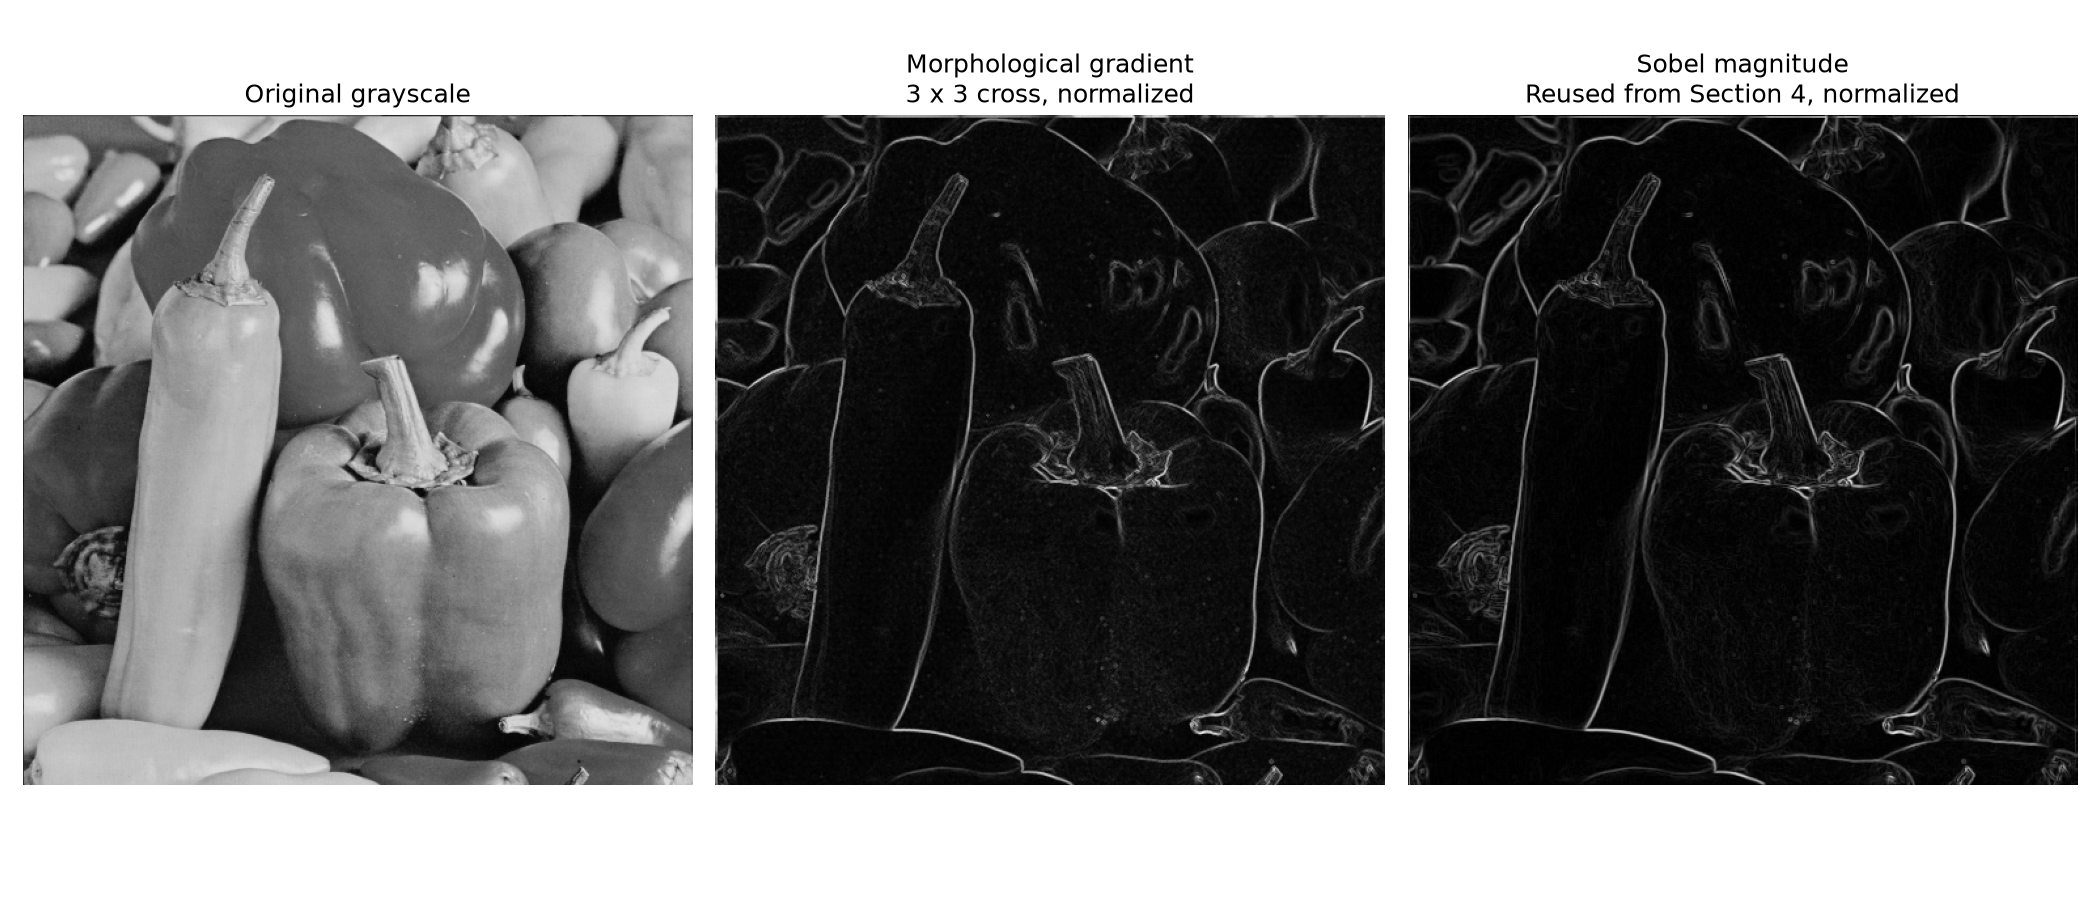
\includegraphics[trim=675.84bp 55.2bp 10.56bp 55.2bp,clip,width=\linewidth]{section11_gradient_comparison.png}
\end{minipage}
\caption{Low-pass: 0--255; high-pass: \(\pm155.400\), zero middle gray;
gradients: 0--255, normalized separately.}
\label{fig:frequency}
\end{figure}

\subsection{Histograms and Image Enhancement}
\textbf{Q9.1.} The normalized histogram summed to 1: 76.43\% of pixels were
64--191, with the highest bar at 96 and another group around 150--190;
the maximum was 228. Cumulative proportions were 52.51\% at 127 and 92.19\%
at 191, reaching 1 at 228. These describe intensity amounts, not positions.
We used \texttt{[0,256]} because OpenCV excludes the upper limit.

\textbf{Q9.2.} Applying \(128+0.5(I-128)\) in floating point shrank 0--228 to
64--178. The lookup \(T(r)=255\,\mathrm{CDF}(r)\), converted to \texttt{uint8},
restored 0--255; OpenCV's \texttt{equalizeHist()} did too
(Figure~\ref{fig:equalization}). Details became clearer than the flat input;
dark gaps and highlights were stronger than originally, with more visible grain.
Results differed by at most 1 level, mean 0.443756: OpenCV subtracts the first
nonzero cumulative value and rounds, while our method truncates the lab's formula.

\begin{figure}[H]
\centering
\begin{minipage}[b]{0.23\linewidth}\centering\small Original\\[2pt]
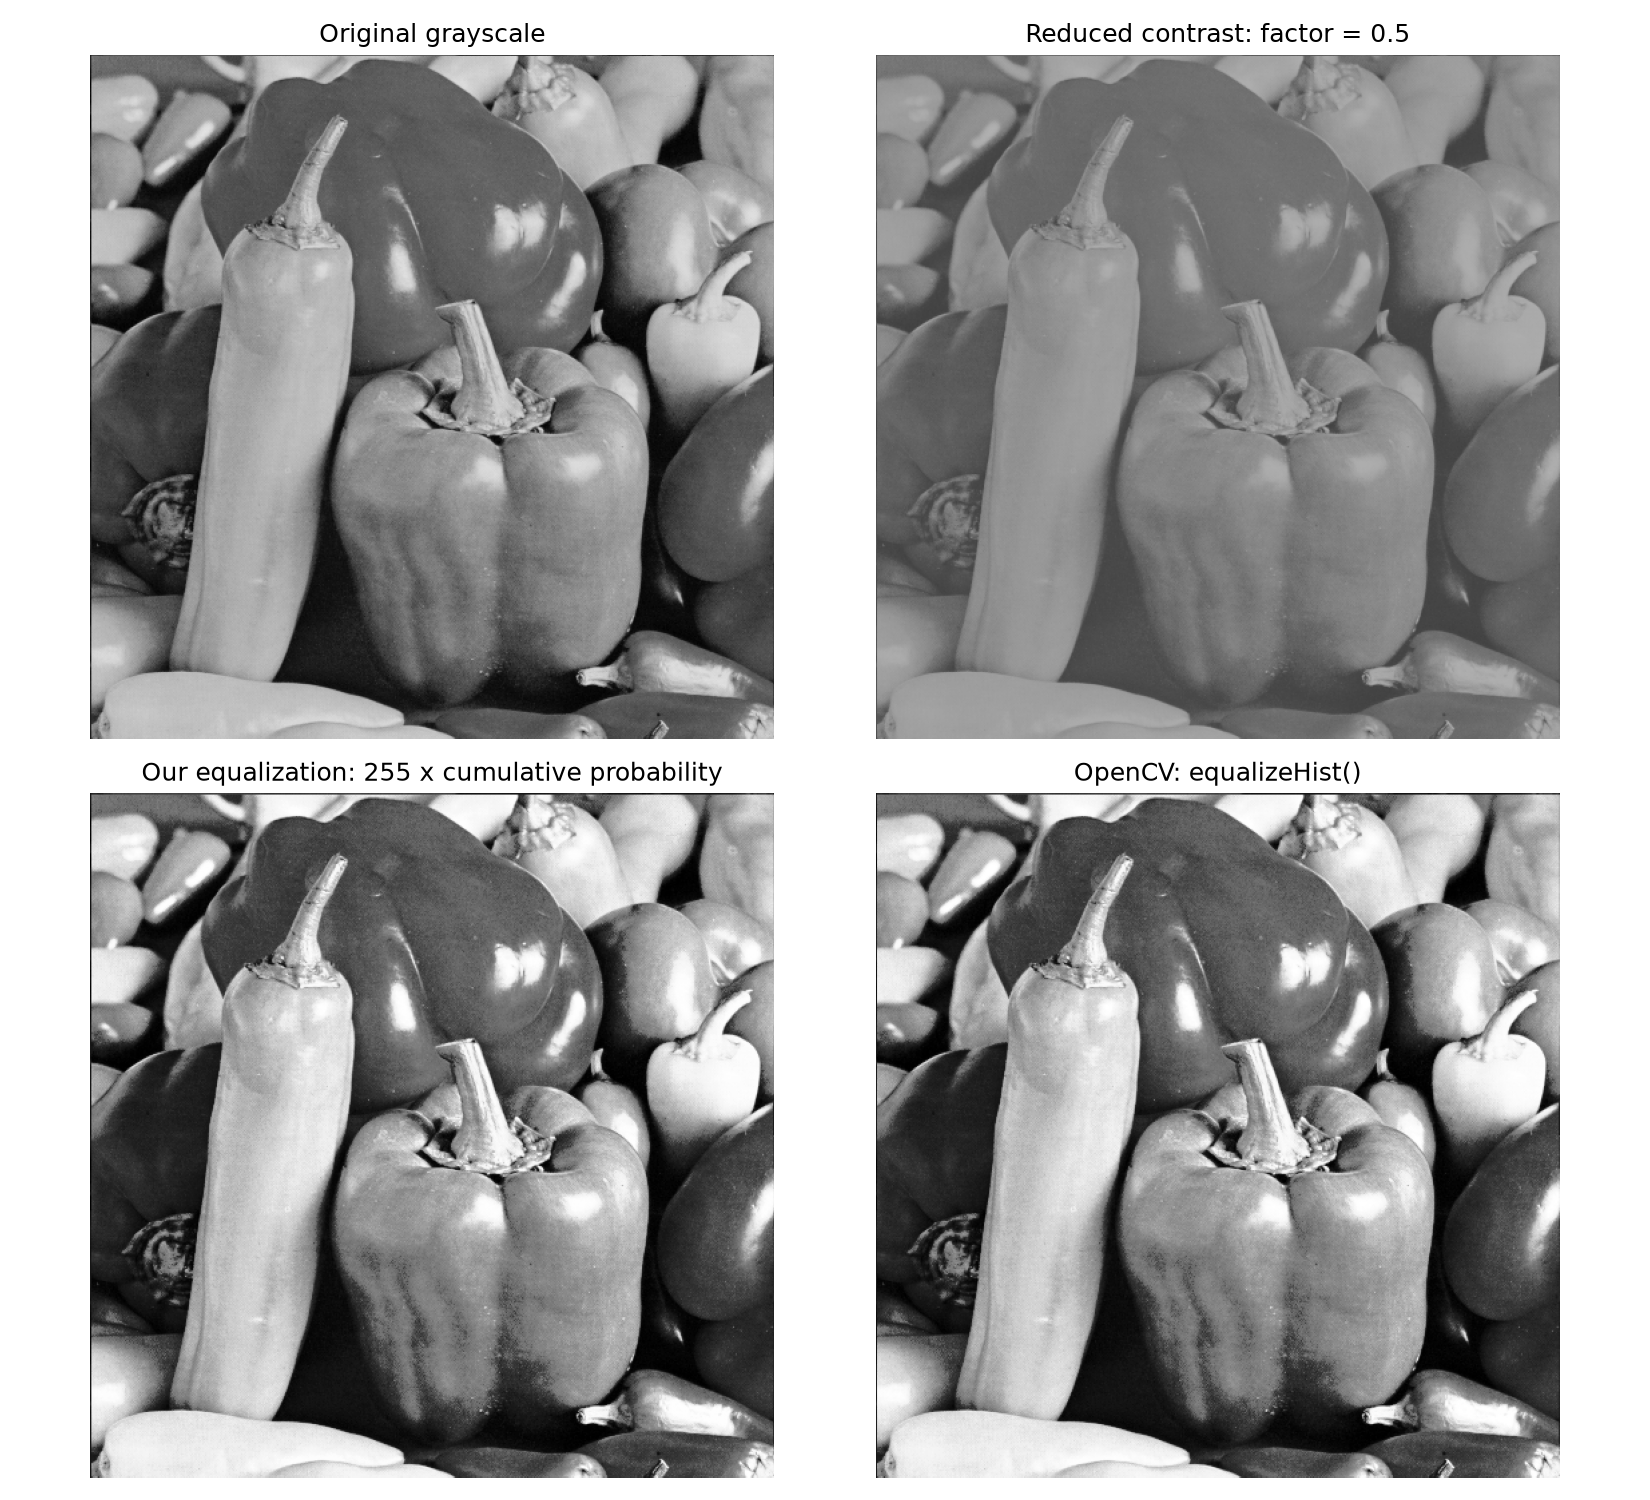
\includegraphics[trim=43.2bp 365.28bp 420.48bp 26.4bp,clip,width=\linewidth]{section9_histogram_equalization.png}
\end{minipage}\hfill
\begin{minipage}[b]{0.23\linewidth}\centering\small Contrast 0.5\\[2pt]
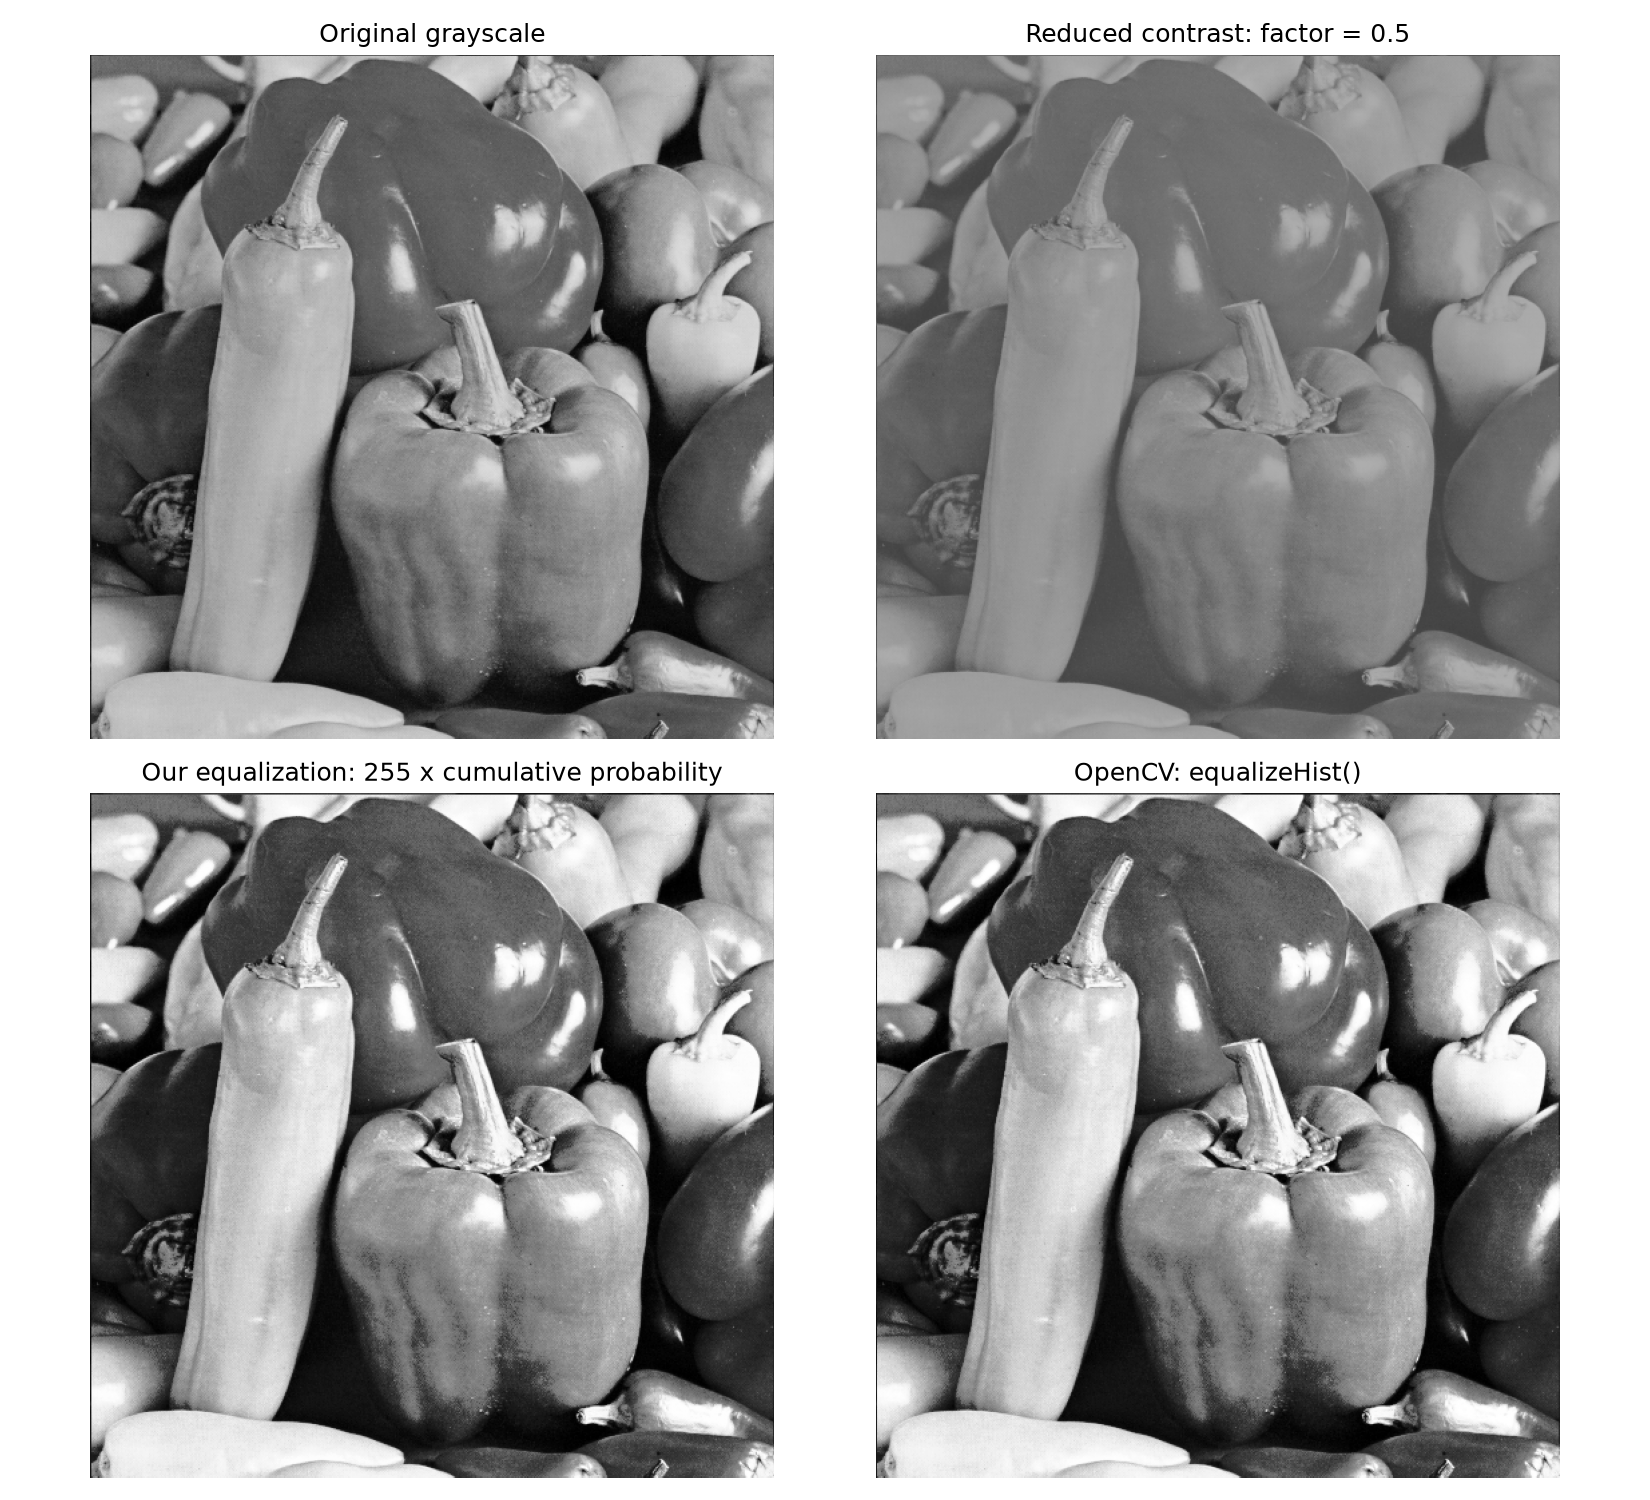
\includegraphics[trim=420.48bp 365.28bp 43.2bp 26.4bp,clip,width=\linewidth]{section9_histogram_equalization.png}
\end{minipage}\hfill
\begin{minipage}[b]{0.23\linewidth}\centering\small CDF method\\[2pt]
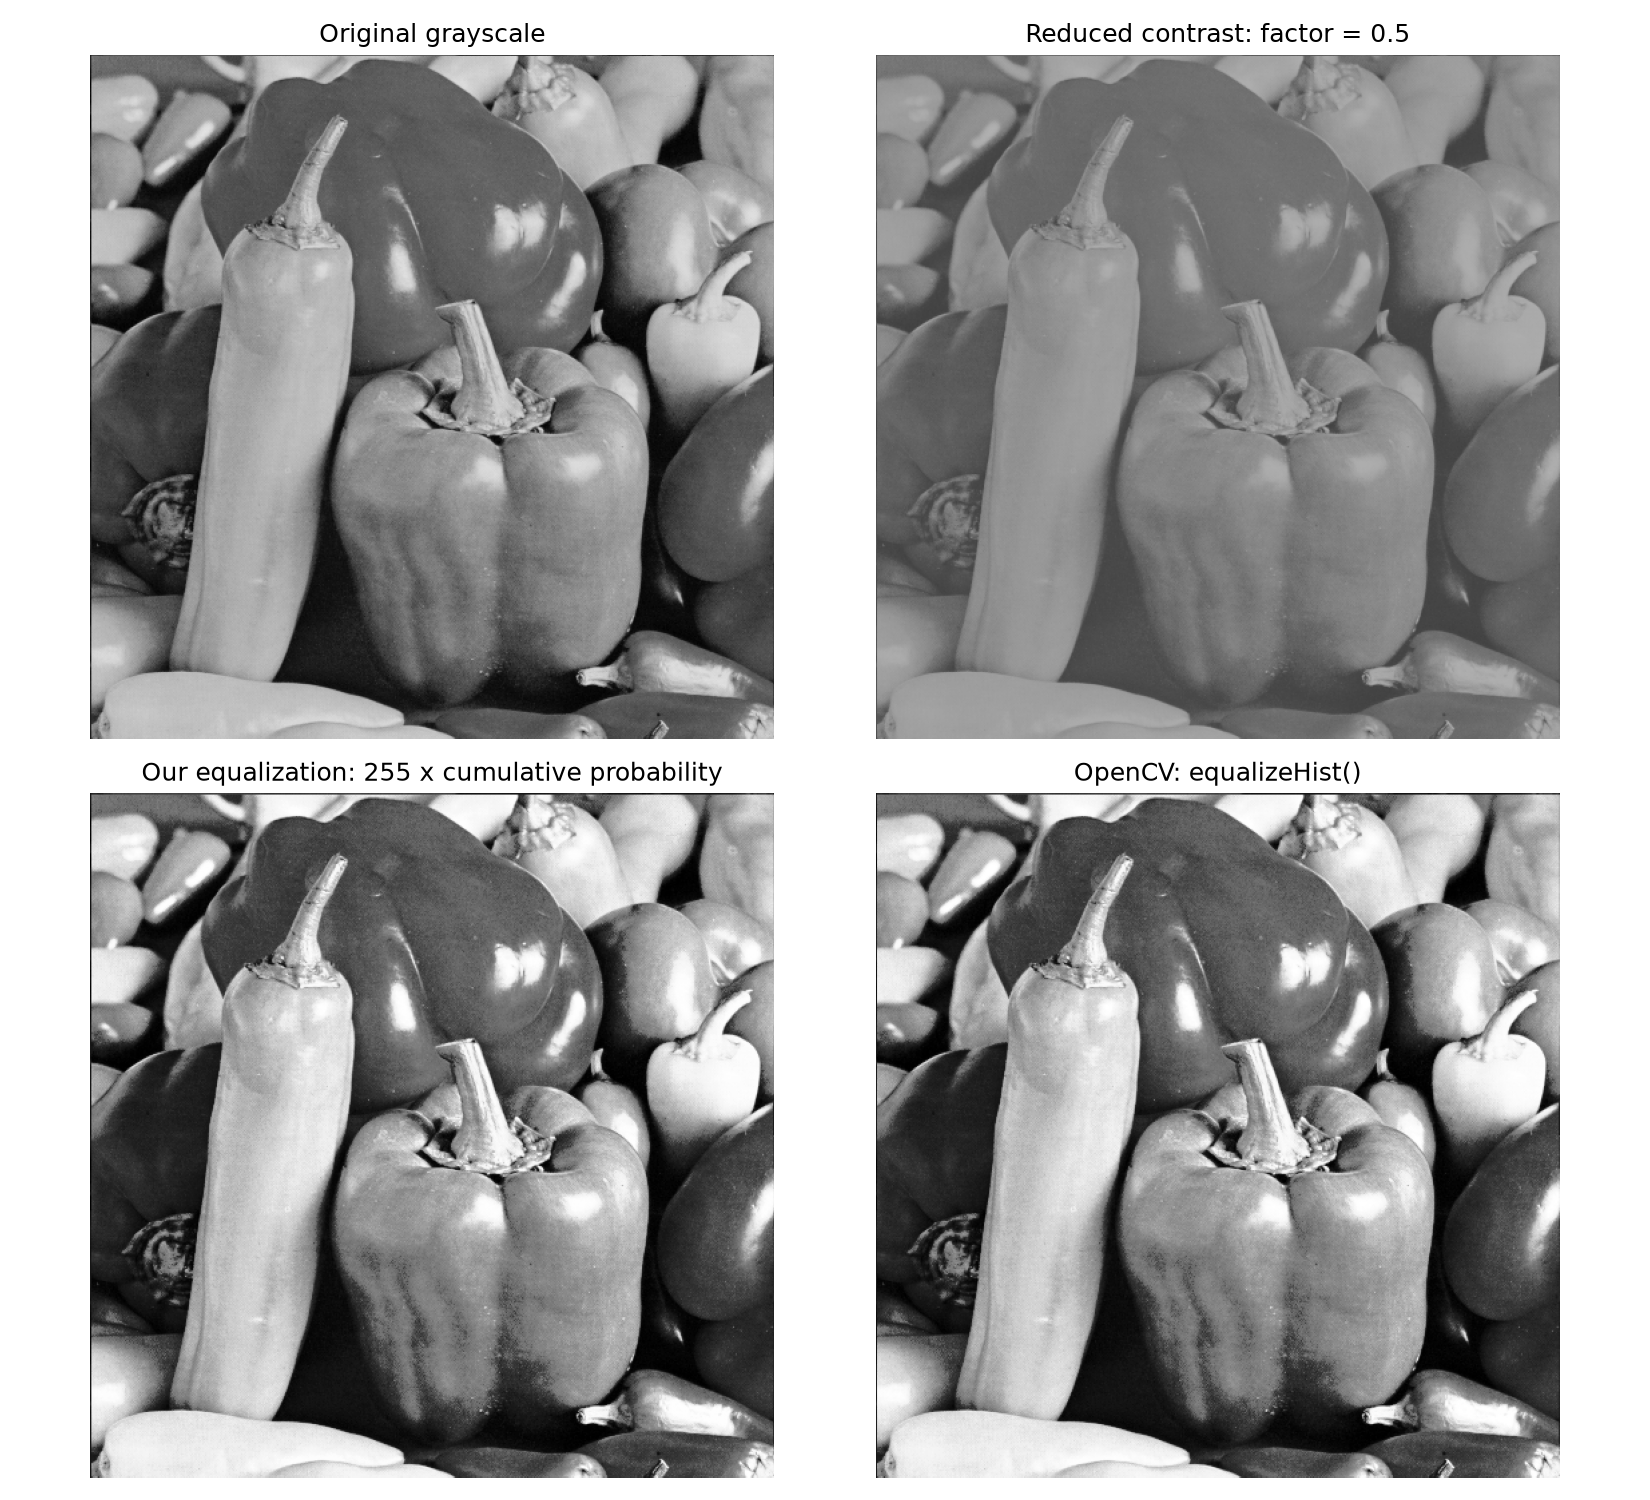
\includegraphics[trim=43.2bp 10.56bp 420.48bp 381.12bp,clip,width=\linewidth]{section9_histogram_equalization.png}
\end{minipage}\hfill
\begin{minipage}[b]{0.23\linewidth}\centering\small OpenCV\\[2pt]
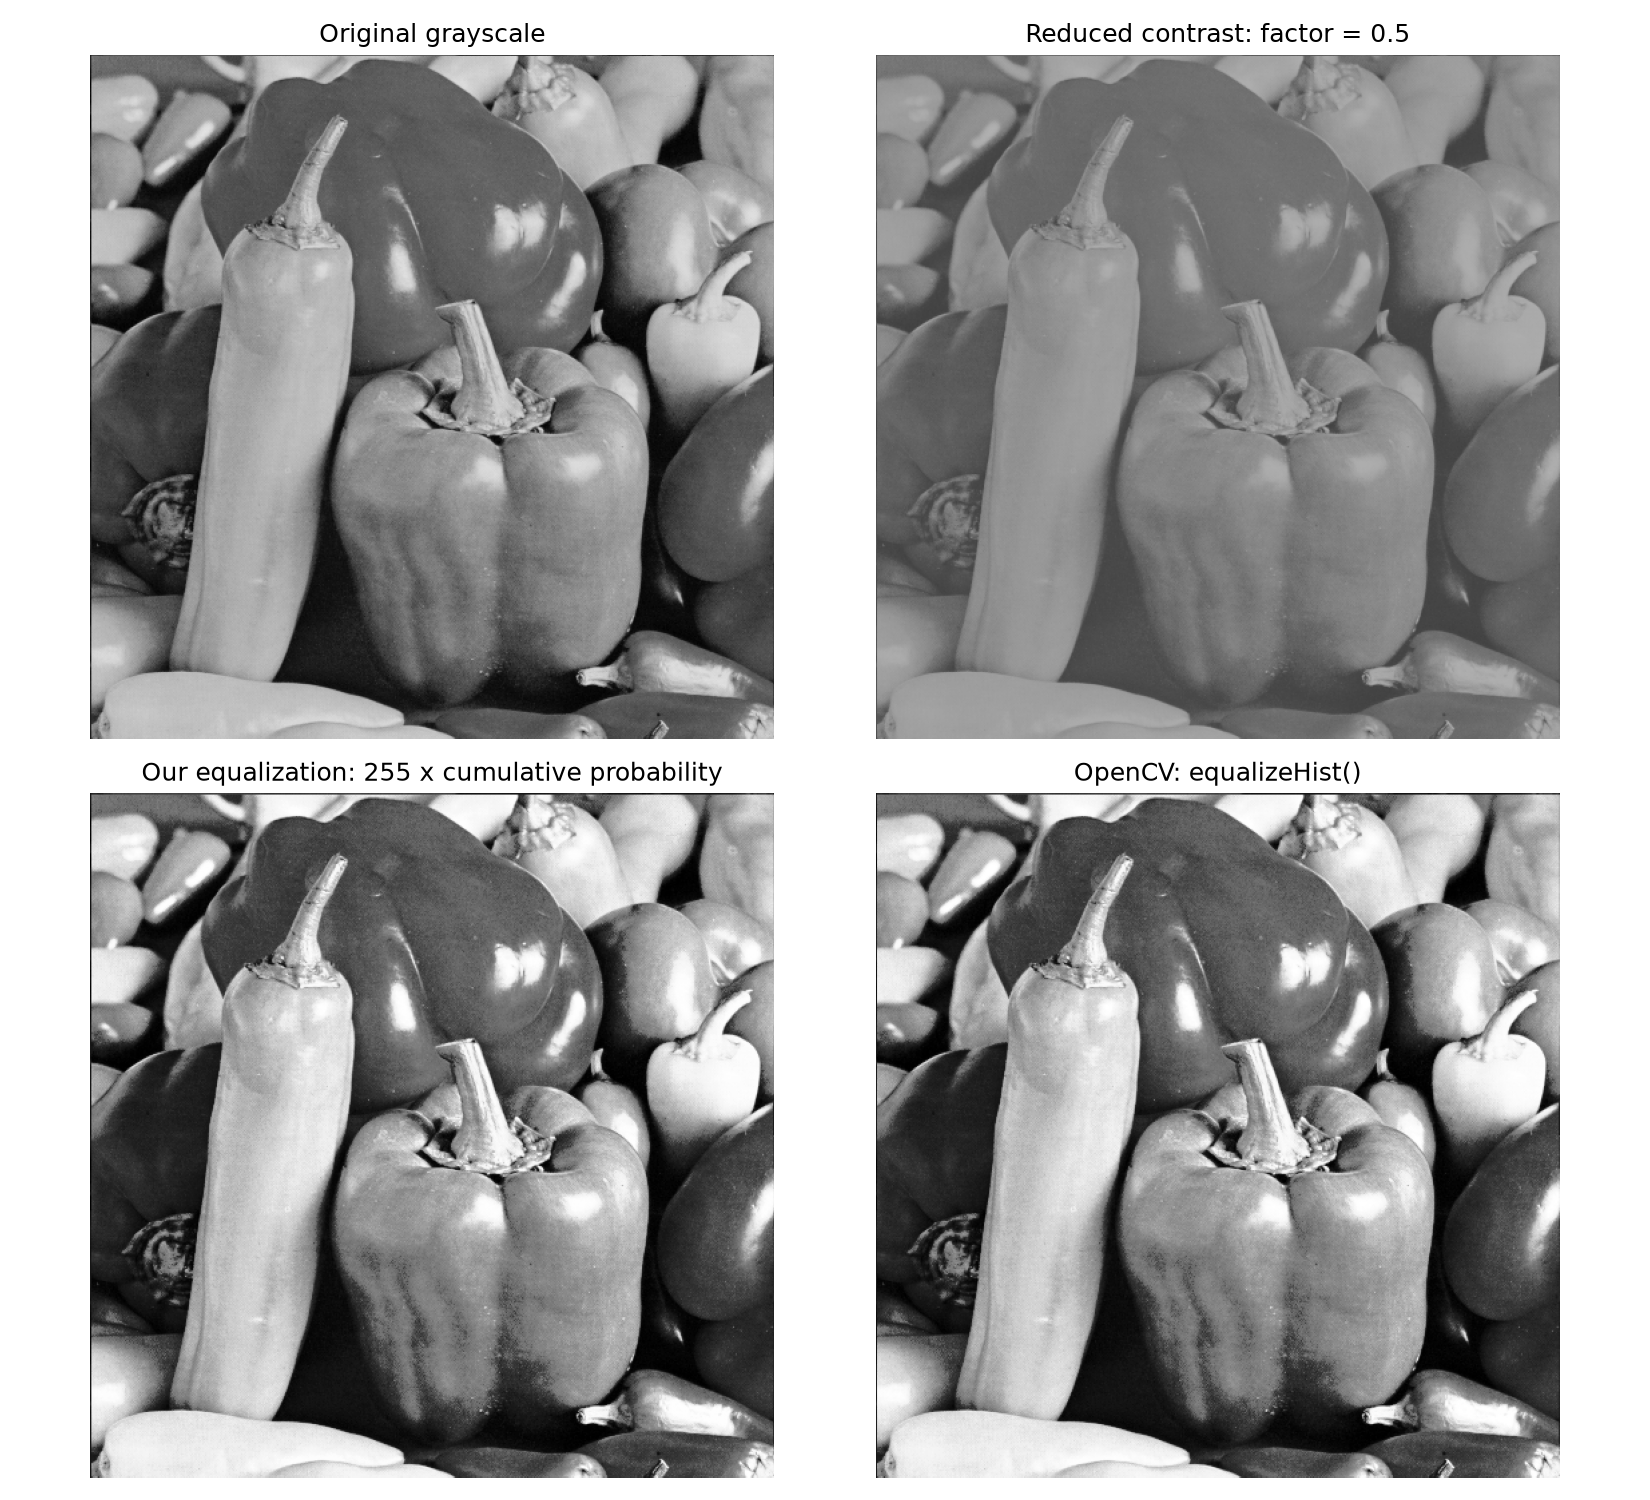
\includegraphics[trim=420.48bp 10.56bp 43.2bp 381.12bp,clip,width=\linewidth]{section9_histogram_equalization.png}
\end{minipage}
\caption{Contrast reduction and equalization. All four panels use 0--255.}
\label{fig:equalization}
\end{figure}

\subsection{Noise and Noise Reduction}
\textbf{Q10.1.} With seed 42, one zero-mean Gaussian sample was scaled and added
in floating point, then clipped before integer conversion. Median \(3\times3\)
at noise \(\sigma=25\) changed PSNR from 20.318 to 26.829 dB; bilateral
(diameter 9, colour/spatial sigmas 75/75) at \(\sigma=35\) changed 17.519 to
26.888 dB. The 0.059 dB gap closely matched outputs, but different input noise
prevents a same-input ranking. Bilateral trials at \(\sigma=25,30,35\) gave
28.860, 28.004, 26.888 dB. Both reduced grain; bilateral looked smoother but
softened stems. Similar PSNR did not mean identical appearance.

\textbf{Q10.2.} Both \(3\times3\) filters received the same noisy image for each
row of Table~\ref{tab:noise}. Salt-and-pepper probability was 4\% total
(2\% black, 2\% white without overlap); 3.986\% of pixels were selected.
Mean filtering gave slightly better Gaussian results but blurred edges.
Median removed isolated extremes much better; mean filtering spread them
into gray marks. \texttt{cv2.PSNR()} used the clean image, with differences from unrounded values.

\begin{table}[H]
\centering\small
\caption{Same-input filtering: PSNR and mean-minus-median difference, all in dB.}
\label{tab:noise}
\begin{tabular}{lrrrr}\toprule
Noise & Input & Mean & Median & Difference\\\midrule
Gaussian, \(\sigma=25\) & 20.318 & 27.237 & 26.829 & \(+0.409\)\\
Salt-and-pepper, 4\% & 19.296 & 26.516 & 34.035 & \(-7.519\)\\\bottomrule
\end{tabular}
\end{table}

\subsection{Morphological Filtering}
\textbf{Q11.1.} Two \(128\times128\) binary tests used separated shapes:
A had a circle, rectangle and triangle; B had two circles of different sizes,
a rectangle and triangle. Each included three white specks and a \(2\times2\)
black hole. Opening with a \(3\times3\) cross removed specks; closing with a
\(5\times5\) ellipse filled the hole. Eight-connected labels minus background
gave expected/detected counts 3/3 and 4/4. Corners rounded slightly; touching
objects would count together.

\textbf{Q11.2.} Dilation minus erosion with the cross gave pepper boundaries
and more surface grain; Sobel outlines looked smoother (Figure~\ref{fig:frequency}, right pair).
Raw ranges were 0--204 and 0--812.857, each separately displayed as 0--255:
display brightness is not comparable raw strength. Morphology suits binary
shapes and kernel-dependent boundaries; Sobel suits grayscale brightness changes
and directional derivatives. Its magnitude alone shows strength, not direction.

\section{Discussion}
Vectorization and lookup saved time without changing outputs. Fewer operations
did not guarantee faster Gaussian filtering; these recorded timings describe
one computer run. Filtering traded noise against detail and depended on noise
type. Equalization exposed grain as well as detail. The three-image fit and
touching-object limitation show why the chosen representation and settings matter.

\section{Conclusion}
The experiments linked pixel values, colour, spatial detail and frequency content.
Numerical comparisons supported the visual results, while timing, memory and
noise comparisons helped explain practical trade-offs.

\section*{Appendix: Code Snippets}
\small
\textbf{FFT filtering.} The circular mask keeps low frequencies; the inverse FFT returns the smooth image.
\lstinputlisting[firstline=512,lastline=514]{../lab3.py}
\textbf{Object counting, inside the loop.} Count connected regions and exclude the background.
\lstinputlisting[firstline=738,lastline=739]{../lab3.py}
\end{document}
